%%%%%%%%%%%%%%%%%%%%%%%%%%%%%%%%%%%%%%%%%
% Version 2.0 (10/10/16)
%
% Original author:
% Frits Wenneker (http://www.howtotex.com)
% Modifier:
% Altug Yildirim
%
% License:
% CC BY-NC-SA 3.0 (http://creativecommons.org/licenses/by-nc-sa/3.0/)
%
%%%%%%%%%%%%%%%%%%%%%%%%%%%%%%%%%%%%%%%%%

%----------------------------------------------------------------------------------------
%	PACKAGES AND OTHER DOCUMENT CONFIGURATIONS
%----------------------------------------------------------------------------------------

\documentclass[paper=a4, fontsize=11pt]{scrartcl} % A4 paper and 11pt font size

\usepackage[T1]{fontenc} % Use 8-bit encoding that has 256 glyphs
\usepackage{fourier} % Use the Adobe Utopia font for the document - comment this line to return to the LaTeX default
\usepackage[english]{babel} % English language/hyphenation
\usepackage{amsmath,amsfonts,amsthm} % Math packages
\usepackage{adjustbox} %for adjusting the table size
\usepackage[affil-it]{authblk}  %for adjusting the author and affilition font size
\usepackage[font=scriptsize]{caption} %for adjusting the font size of captions
\usepackage{multirow} %for merging the header cells
\usepackage{hhline} %for merging the header cells
\usepackage{listings} %for code display
\usepackage{color} %for code display
\usepackage{subfig}
\lstset{frame=tb,
  language=Matlab,
  aboveskip=3mm,
  belowskip=3mm,
  showstringspaces=false,
  columns=flexible,
  basicstyle={\small\ttfamily},
  numbers=none,
  numberstyle=\tiny\color{gray},
  keywordstyle=\color{blue},
  commentstyle=\color{red},
  stringstyle=\color{green},
  breaklines=true,
  breakatwhitespace=true,
  tabsize=1
} %for code didplay

\usepackage{graphicx} %for inserting graphics
\graphicspath{ {images/} } %for determining the folder where the graphic is

\usepackage{sectsty} % Allows customizing section commands
\allsectionsfont{\centering \normalfont\scshape} % Make all sections centered, the default font and small caps
\newif\ifcomment
\commenttrue %Show comments

\renewcommand\Authfont{\fontsize{12}{14.4}\selectfont}
\renewcommand\Affilfont{\fontsize{9}{10.8}\itshape}

\usepackage{fancyhdr} % Custom headers and footers
\pagestyle{fancyplain} % Makes all pages in the document conform to the custom headers and footers
\fancyhead{} % No page header - if you want one, create it in the same way as the footers below
\fancyfoot[L]{} % Empty left footer
\fancyfoot[C]{} % Empty center footer
\fancyfoot[R]{\thepage} % Page numbering for right footer
\renewcommand{\headrulewidth}{0pt} % Remove header underlines
\renewcommand{\footrulewidth}{0pt} % Remove footer underlines
\setlength{\headheight}{13.6pt} % Customize the height of the header

\numberwithin{equation}{section} % Number equations within sections (i.e. 1.1, 1.2, 2.1, 2.2 instead of 1, 2, 3, 4)
\numberwithin{figure}{section} % Number figures within sections (i.e. 1.1, 1.2, 2.1, 2.2 instead of 1, 2, 3, 4)
\numberwithin{table}{section} % Number tables within sections (i.e. 1.1, 1.2, 2.1, 2.2 instead of 1, 2, 3, 4)

\setlength\parindent{0pt} % Removes all indentation from paragraphs - comment this line for an assignment with lots of text

%----------------------------------------------------------------------------------------
%	TITLE SECTION
%----------------------------------------------------------------------------------------

\newcommand{\horrule}[1]{\rule{\linewidth}{#1}} % Create horizontal rule command with 1 argument of height

\title{	
\normalfont \normalsize 
\textsc{\.{I}stanbul Teknik \"Universitesi, Matematik B\"ol\"um\"u \\ Kismi T\"urevli Diferansiyel Denklemler i\c{c}in Sayisal Analiz I} \\ [25pt]
\horrule{0.5pt} \\[0.4cm] % Thin top horizontal rule
\large \"Odev III \\ % The assignment title
\horrule{0.5pt} \\[0.4cm] % Thick bottom horizontal rule
}

\author{Haydar Altu\u{g} Y{\i}ld{\i}r{\i}m \\ 509161108} 

\date{\normalsize\today} % Today's date or a custom date

\begin{document}

\maketitle % Print the title
%This part is for using the section properties without having the headline
\newcommand\invisiblesection[1]{%
  \refstepcounter{section}%
  \addcontentsline{toc}{section}{\protect\numberline{\thesection}#1}%
  \sectionmark{#1}}
\invisiblesection{Blah}

%\section{Numerical and Analytical Solution for Hat Equation with Dirichlet Boundary Condition}

1)Analitik \c{c}\"oz\"um\"u bul ve \c{c}izdir\\
2)Euler \c{s}emas{\i}=20

\begin{align}
u_t=u_xx\\
u(0,t)=u(1,t)=0 \\
u^0(x)= 2x if 0 \leqslant x \leqslant 1/2 \\
u^0(x)= 2-2x if 1/2 \leqslant x \leqslant 1 \\
\end{align}

\ifcomment
N\"umerik ve analitik \c{c}\"oz\"um i\c{c}in yaz{\i}lm{\i}\c{s} kod;

\begin{lstlisting}
clear all;
clc;
%numerical solution
%%%%%%%%%%%%%%%%%%%%%%%%%%%%%%%%%%%%%
%defining the Dx
dx=1/20;
t=40;
%defining Dt 
dt=0.0012; 
%dt=0.0013;

%defining mu
mu=dt/(dx)^2;

%creating the mesh grid for 1D and defining the boundary conditions for x
x_num=0:dx:1;

%creating array for 
u= zeros(1,length(x_num));

%initial conditions for u(x)
for k=1:length(x_num)
  if (x_num(k)<0.5)
    u(k)=2*x_num(k);
  else (x_num(k)>=0.5);
    u(k)=2-2*x_num(k);
  end
end

%boundary conditions for u(x)
u(1)= 0;
u(length(x_num))=0;

%calculating Euler scheme
for n=1:t
  for j=2:(length(x_num)-1)
    u(j)=u(j)+mu*(u(j+1)-2*u(j)+u(j-1));
   end
  u(1)= 0;
  u(length(x_num))=0;
end
%%%%%%%%%%%%%%%%%%%%%%%%%%%%%%%%%%%%%

%analytical solution
%%%%%%%%%%%%%%%%%%%%%%%%%%%%%%%%%%%%%
x_space=0:dx:1; %creating space for analytical solution
u_analytical=zeros(1,length(x_space)); %solution u(x,t)
g=0; %single point for u(x,t)
syms x;
for m=1:length(x_space) %calculating every single u(x,t) value for plotting
    for k=1:6 %this loop represents the sum in the analytical solution
        %fourier coefficient symbolic solution
        F=int(4*x*sin(pi*k*x),0,0.5)+int(2*(2-2*x)*sin(pi*k*x),0.5,1);
        %calculating u(x,t) for single point in mesh
        g=g+double(F*sin(k*pi*x_space(m))*exp(-((k*pi)^2)*t)); 
    end
    %creating the array for plotting
    u_analytical(m)=g;
end
%%%%%%%%%%%%%%%%%%%%%%%%%%%%%%%%%%%%%
%The analytical part simply do not work but I could not understand the
%reason thus there is only numerical part that is plotted.
plot (x_num,u);
\end{lstlisting}
\fi
N\"umerik \c{c}\"oz\"um\"un farkl{\i} $\Delta$t ve zaman aral{\i}klar{\i} i\c{c}in grafikleri;

\begin{figure}[h]
\centering
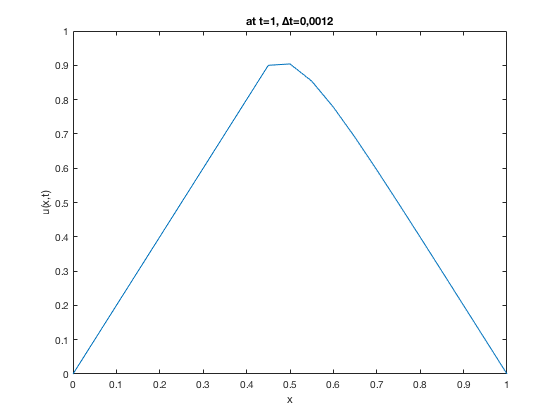
\includegraphics[scale=0.5]{graph1}
\end{figure}
\begin{figure}[h]
\centering
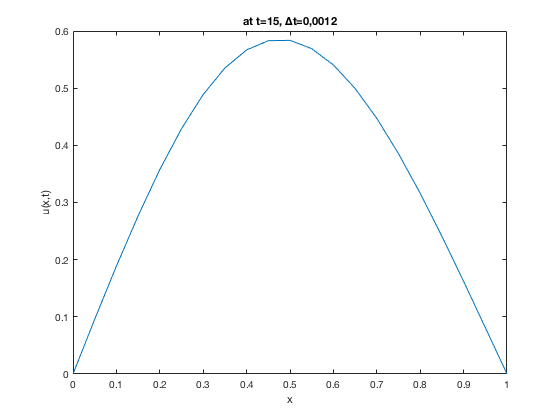
\includegraphics[scale=0.5]{graph2}
\end{figure}
\begin{figure}[h]
\centering
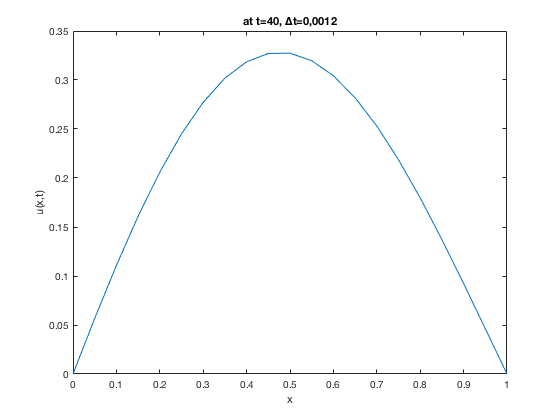
\includegraphics[scale=0.6]{graph3}
\end{figure}
\begin{figure}[h]
\centering
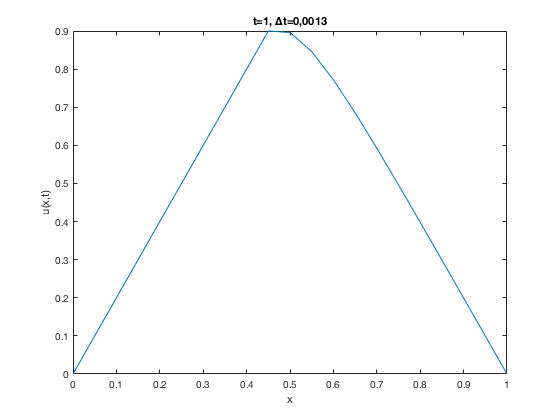
\includegraphics[scale=0.6]{graph4}
\end{figure}
\begin{figure}[h]
\centering
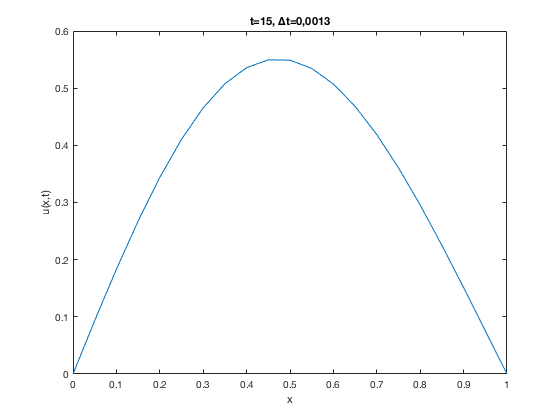
\includegraphics[scale=0.6]{graph5}
\end{figure}
\begin{figure}[h]
\centering
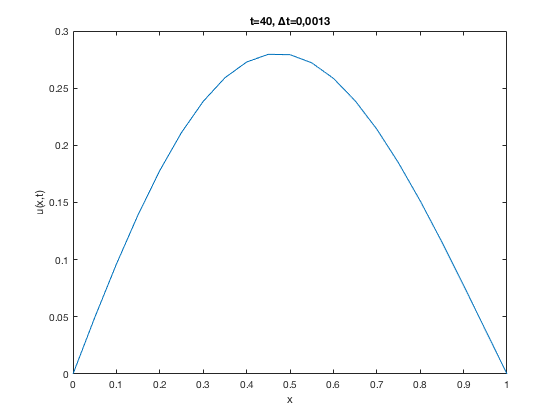
\includegraphics[scale=0.6]{graph6}
\end{figure}
\end{document}